\documentclass[11pt]{article}

\usepackage{geometry}
 \geometry{
 letterpaper,
 left=1in,
 right=1in,
 bottom=1in,
 top=1.25in
 }               % See geometry.pdf to learn the layout options. There are lots.
%\geometry{landscape}                
\usepackage{graphicx}
\usepackage{amssymb}
\usepackage{epstopdf}
\DeclareGraphicsRule{.tif}{png}{.png}{`convert #1 `dirname #1`/`basename #1 .tif`.png}
\usepackage{url}
\usepackage{amsmath}
\usepackage{mathtools}
\usepackage{booktabs}
\usepackage[format=hang,labelfont=bf]{caption}
\usepackage{float}
\usepackage[parfill]{parskip}
\usepackage{tensor}
\usepackage{natbib}
\usepackage[inline]{enumitem}
%\begin{enumerate*}%[label=\textit{\alph*)}] 
%\item
%\end{enumerate*} 
\usepackage{color}

% Appendices - nice table/figure numbering with appendix identifier
\usepackage[titletoc,toc,title]{appendix}
%% Restart table/figure numbering in appendices using <\counterwithin{figure}{section}>
%\usepackage{chngcntr}

\usepackage[parfill]{parskip}

\usepackage{url}
%\usepackage{hyperref}
\usepackage{authblk}
\renewcommand\Affilfont{\footnotesize}
\usepackage{easymat}
\usepackage{bigstrut}
\usepackage{threeparttable} 
\usepackage[format=hang,labelfont=bf]{caption}
\usepackage{rotating}
\usepackage{subfig}
\usepackage{wrapfig}
\usepackage{mdframed}
\usepackage[raggedright]{titlesec}
\usepackage{longtable}

\usepackage{array}
\newcolumntype{L}[1]{>{\raggedright\let\newline\\\arraybackslash\hspace{0pt}}m{#1}}
\newcolumntype{C}[1]{>{\centering\let\newline\\\arraybackslash\hspace{0pt}}m{#1}}
\newcolumntype{R}[1]{>{\raggedleft\let\newline\\\arraybackslash\hspace{0pt}}m{#1}}

\usepackage{scrextend}
\deffootnote[1em]{1em}{1em}{\textsuperscript{\thefootnotemark}}

\usepackage[table, dvipsnames]{xcolor}
\definecolor{lightgray}{gray}{0.95}
\definecolor{white}{rgb}{1.0, 1.0, 1.0}

% for making changes in response to reviews
% must come *after* xcolor
% toggle the following two lines to reveal or hide the changes
%\usepackage[commentmarkup=footnote]{changes}
\usepackage[final]{changes}
\definechangesauthor[name={Reviewer 1}, color=blue]{r1}
\definechangesauthor[name={Reviewer 2}, color=blue]{r2}
\definechangesauthor[name={Reviewer 3}, color=blue]{r3}
\definechangesauthor[name={Reviewer 4}, color=OliveGreen]{r4}
\definechangesauthor[name={Reviewer 5}, color=OliveGreen]{r5}
\definechangesauthor[name={Editors}, color=Violet]{editors}
\definechangesauthor[name={Notes}, color=brown]{note}

\DeclareMathOperator{\Tr}{Tr}

\newcommand{\mbf}{\mathbf}

\newcommand{\qf}{\tensor*[_5]{\mbox{q}}{_0}}
\newcommand{\qoz}{\tensor*[_1]{\mbox{q}}{_0}}
\newcommand{\qoo}{\tensor*[_1]{\mbox{q}}{_1}}
\newcommand{\qfo}{\tensor*[_4]{\mbox{q}}{_1}}
\newcommand{\qof}{\tensor*[_1]{\mbox{q}}{_4}}
\newcommand{\qff}{\tensor*[_{45}]{\mbox{q}}{_{15}}}
\newcommand{\qox}{\tensor*[_{1}]{\mbox{q}}{_{x}}}
\newcommand{\qoa}{\tensor*[_{1}]{\mbox{q}}{_{a}}}
\newcommand{\qfx}{\tensor*[_{5}]{\mbox{q}}{_{x}}}
\newcommand{\qnx}{\tensor*[_{n}]{\mbox{q}}{_{x}}}
\newcommand{\qts}{\tensor*[_{20}]{\mbox{q}}{_{60}}}
\newcommand{\qfxhat}{\tensor*[_{5}]{\widehat{\mbox{q}}}{_{x}}}

\newcommand{\ez}{{\mbox{e}}{_0}}
\newcommand{\ezhat}{{\widehat{\mbox{e}}}{_0}}
\newcommand{\ex}{{\mbox{e}}{_x}}
\newcommand{\exhat}{{\widehat{\mbox{e}}}{_x}}

\newcommand{\mfx}{\tensor*[_{5}]{\mbox{m}}{_{x}}}
\newcommand{\mfz}{\tensor*[_{5}]{\mbox{m}}{_{0}}}

\newcommand{\anx}{\tensor*[_{n}]{\mbox{a}}{_{x}}}
\newcommand{\aoz}{\tensor*[_{1}]{\mbox{a}}{_{0}}}
\newcommand{\alast}{\tensor*[_{+}]{\mbox{a}}{_{110}}}

\newcommand{\lx}{\tensor*[_{}]{\mbox{l}}{_{x}}}

\newcommand{\logit}{\mbox{logit}}
\newcommand{\expit}{\mbox{expit}}

% Insert labels and numbers into complex align environment equations, e.g. matrices of equations
\makeatletter
\newcommand\Label[1]{&\refstepcounter{equation}(\theequation)\ltx@label{#1}&}
\makeatother

%double space
\usepackage{setspace}
%\linespread{1.5}

%touch-up footnote formatting
\usepackage{scrextend}
\deffootnote[1em]{1em}{1em}{\textsuperscript{\thefootnotemark}}

%% Fonts
% sans-serif
\renewcommand{\familydefault}{\sfdefault}
% Helvetica
\usepackage{helvet}
% mathmode fonts sans-serif too
\usepackage[italic]{mathastext}
% 'isomath' sets upper case greek letters italic in accordance with 
% the International Standard ISO 80000-2
\usepackage{isomath}

\sloppy

% remove extra spaces after using \input{}
\newcommand{\lineinput}[1]{%
  \begingroup\endlinechar=-1 \input{#1}\endgroup
}

% reference the appendices in separate file
\usepackage{xr}
\externaldocument{"SVD-Comp-Appendices"}

% define variable for number of life tables per sex
\DeclareRobustCommand{\LTtot}{\input{../tables/LTtot.txt}}

% define variable for number of life tables for both sexes
\DeclareRobustCommand{\LTtotBoth}{\input{../tables/LTtotBoth.txt}}

% define variable for date when HMD downloaded
\DeclareRobustCommand{\HMDdate}{ \begingroup\endlinechar=-1 \input{../tables/HMDdate.txt}\endgroup}




\title{\vfill A General Age-Specific Mortality Model with An Example Indexed by Child or Both Child and Adult Mortality}

\author[1,2,*]{Samuel J. Clark}

\affil[1]{Department of Sociology, The Ohio State University}
\affil[2]{MRC/Wits Rural Public Health and Health Transitions Research Unit (Agincourt), School of Public Health, Faculty of Health Sciences, University of the Witwatersrand}
\affil[*] {Contact: work@samclark.net, 206.303.9620}

%\date{\today \vfill}
\date{2018 \vfill}

\begin{document}

\pagenumbering{roman} 
\maketitle

%\thispagestyle{empty}

%\newpage
%\listofchanges

\newpage
\begin{abstract}
\noindent The majority of countries in Africa and nearly one third of all countries require mortality models to infer the complete age schedules of mortality that are required to conduct population estimates, projections/forecasts, and other tasks in demography and epidemiology.  Models that relate child mortality to mortality at other ages are important because almost all countries have measures of child mortality. A general, parametrizable component model of mortality is defined using the singular value decomposition (SVD-Comp) and calibrated to the relationship between child or child/adult mortality and mortality at other ages in the observed mortality schedules of the Human Mortality Database.  Cross validation is used to validate the model, and the predictive performance of the model is compared to that of the Log-Quad model, designed to do the same thing. Prediction and cross validation tests indicate that the child mortality-calibrated SVD-Comp is able to accurately represent the observed mortality schedules in the Human Mortality Database, is robust to the selection of mortality schedules used to calibrate it, and performs better than the Log-Quad Model.  The child mortality-calibrated SVD-Comp can be used where child mortality is available but mortality at other ages is unknown.
\end{abstract}

%\newpage
%\tableofcontents
%\newpage
%\listoftables
%\newpage
%\listoffigures

\clearpage 
\pagenumbering{arabic} 
\newpage


%%% === %%% === %%%
\section{Introduction}

Complete age-specific mortality schedules are necessary inputs to a wide variety of formal demographic and epidemiological methods.  A key example is the biennial World Population Prospects (WPP) \citep{un2015} produced by the UN Population Division.  These are \added{generally} considered the \replaced{reference}{gold standard} population indicators and are widely used by other domestic and international agencies as inputs to estimation and modeling exercises.  The WPP contains estimates of time-sex-age-specific mortality, fertility, and population size from 1950 to the present and forecasts of the same quantities to 2100 for all countries of the world.  Consequently each WPP update must contain full age-specific mortality schedules covering the period 1950--2100.

\begin{table}[htp]
\captionsetup{format=plain,font=normalsize,margin=0.6cm,justification=justified}
\caption{\textbf{Countries or regions with no information on either child or adult mortality.} UN countries and regions that do not have information on either child or adult mortality for the 2015 update of the World Population Prospects, with population and fraction of total population for which information is missing. \textit{Reference:} \cite{unWPPMethods2015} tables I.1b (p 5) and I.1c (p 6).}
\begin{center}
\begin{tabular}{llllllll}

\toprule
 & \multicolumn{3}{c}{Child Mortality} & &  \multicolumn{3}{c}{Adult Mortality} \\
 \cmidrule{2-4} \cmidrule{6-8}
 & Regions & \begin{tabular}{@{}l} Population \\ (millions) \end{tabular} & \begin{tabular}{@{}l} Percent \\ Population \end{tabular} & & Regions & \begin{tabular}{@{}l} Population \\ (millions) \end{tabular} &  \begin{tabular}{@{}l} Percent \\ Population \end{tabular} \\
\midrule
World & 1 & 1 & 0.0\% & & 50 & 973 & 13.2\% \\
Africa & 1 & 1 & 0.0\% & & 33 & 666 & 56.1\% \\

\bottomrule
\end{tabular}
\end{center}
\label{tab:mxMiss}
\end{table}%

Some countries in the developing world, particularly in Africa, do not yet have civil registration and vital statistic systems that function well enough to accurately report on either fertility or mortality.  Focusing on mortality, Table \ref{tab:mxMiss} displays the number of countries or world regions for which there is no information on either child mortality or adult mortality, with Africa broken out.  Because of the exhaustive coverage of household surveys investigating fertility and maternal/child health, essentially the whole world has at least some recent information on child mortality \citep{li2015wppLt}.  In contrast 50 countries around the world with a total population of nearly 1 billion people have no information on adult mortality, with the bulk of those in Africa -- 33 countries with a total population of 666 million people. 

Mortality models are used to solve this problem and produce full age schedules of mortality.  Table \ref{tab:mxMods} describes the number of countries or world regions for which the UN Population Division must use mortality models of some kind to produce either estimates of life expectancy at birth $\ez$ or full age schedules of mortality.  Most African countries require mortality models for both, and globally 38.6\% of countries require a model for $\ez$ and 32.6\% for age-specific mortality.    

\begin{table}[htp]
\captionsetup{format=plain,font=normalsize,margin=2.4cm,justification=justified}
\caption{\textbf{Countries and regions where mortality models are necessary to estimate life expectancy at birth ($\ez$) or age-specific mortality rates (ASMR).} 
Counts of the number of UN countries  and \replaced{areas}{regions} where mortality models were used to generate estimates of $\ez$ or age-specific mortality rates for the 2015 update of the World Population Prospects. \textit{Reference:} \cite{unWPP2015Meta}.  }
\begin{center}
\begin{tabular}{lrrrrrr}

\toprule
&  & \multicolumn{2}{c}{$\ez$} & & \multicolumn{2}{c}{ASMR}  \\
\cmidrule{3-4} \cmidrule{6-7}
& Countries/Regions & Count & Percent & & Count & Percent \\ 
\midrule
World & 233 & 90 & 38.6\% & & 76 & 32.6\% \\
Africa & 58 & 50 & 86.2\% & & 50 & 86.2\% \\

\bottomrule
\end{tabular}
\end{center}
\label{tab:mxMods}
\end{table}

The standard approach to generating complete age schedules of mortality for countries and \replaced{areas}{regions} with insufficient data is to take advantage of the fact that they do have information on child mortality.  Typically, model life tables are used to extrapolate full mortality schedules from $\qf$\replaced{ -- this is what t}{.  T}he UN Population Division \replaced{does (making heavy use of the traditional \cite{coale1966} model life tables)}{uses the Log Quadratic (Log-Quad) model created by \mbox{\cite{wilmoth2012flexible}} and updated by \mbox{\cite{li2015wppLt}} to do this for the many countries and world regions with incomplete mortality data}, and the Institute for Health Metrics and Evaluation (IHME) uses variations on the Modifed Logit (Mod-Logit) model \citep{murray2003} to do the same.  

The commonly used model life table systems -- Regional Model Life Tables and Stable Populations \citep{coale1966}, Life Tables for Developing Countries \citep{united1982model}, Modified Logit Life Table System (Mod-Logit) \citep{murray2003, Wang2013} and Flexible Two Dimensional Mortality Model (Log-Quad) \citep{wilmoth2012flexible} -- combine a specific model structure and defined variable parameters with a set of fixed parameters that summarize the relationships between mortality at different ages in a set of observed life tables.  All are \emph{empirical} models in the sense that they summarize observed mortality and use that summary to produce \replaced{predicted}{arbitrary} mortality schedules that are consistent with observed mortality.  They come in both regional and continuous forms. \replaced[id=r1]{The regional models identify and replicate commonly observed mortality patterns associated with geographic regions (and \textit{de facto} time periods) and allow mortality to vary continuously within each region-specific pattern.  In contrast the continuous models generate mortality patterns that vary smoothly. Both approaches are essentially two-parameter models.  The regional models first identify a discrete region and then use effectively continuously varying life expectancy within each region to adjust the level of region-specific mortality. The continuous models have two continuously varying parameters, e.g. life expectancy, child mortality, or adult mortality.}
{The regional models identify and replicate commonly observed mortality patterns associated with geographic regions (and \textit{de facto} time periods) while the continuous models generate mortality patterns that vary smoothly. The input parameters range from region and life expectancy to child and adult mortality.} 

\cite{murray2003} enumerate three characteristics required of mortality models: 
\begin{enumerate*}[label=\arabic*)]
\item simplicity and ease of use,
\item comprehensive representation of the true variability in sex-age-specific mortality observed in real populations, and
\item validity that is well quantified by comparing age schedules of mortality predicted by the model to corresponding observed life tables
\end{enumerate*}.
To those I would add:
\begin{enumerate*}[label=\arabic*)]
\item generality with respect to the underlying model structure, 
\item flexibility in terms of input parameters, and 
\item an ability to handle \replaced{a wide range of age groups}{arbitrary}, including very fine-grained, \deleted{age groups} without having to fundamentally alter the structure of the model
\end{enumerate*}. 

This work \added[id=r4]{defines and describes a new SVD component-based} mortality modeling framework that satisfies all of those requirements.  \added[id=r4]{The SVD-component framework provides a general, flexible way to model any demographic age schedule as a function of covariates or predictors that are related to age-specific variation in the age schedule.  Here the SVD-component framework is demonstrated by creating} a mortality model that predicts single-year of age mortality schedules using either $\qf$ or both $\left(\qf, \, \qff \right)$ as predictors, similar to both the Mod-Logit and Log-Quad models.   The resulting model can be used to produce single year of age mortality schedules from $\qf$ alone that are consistent with observed mortality schedules, and this could be useful for those like the UN Population Division who must manipulate full age schedules of mortality but only have observed values for $\qf$.  \added[id=r4]{The resulting SVD-component model performs better than the current state of the art two-parameter model (Log-Quad), provides predictions by single-year of age, and is easily extensible to include additional predictors beyond child and adult mortality.}

The remainder of this article
\begin{enumerate*}[label=\arabic*)]
\item reviews existing mortality models with an emphasis on those that use a dimension-reduction approach, 
\item identifies and describes the empirical life tables used to develop the model,
\item develops and calibrates the model so that it reflects observed mortality across a wide range of settings and times,
\item uses a cross-validation approach to validate the model,
\item compares the performance of the model with that of the Log-Quad model, and
\item presents an example application to mortality data from two developing countries
\end{enumerate*}.


%%% === %%% === %%%
\section{Mortality Models}

Traditional model life tables \citep[e.g.][]{united1955age, ledermann1969nouvelles, coale1966, united1982model, murray2003, wilmoth2012flexible, Wang2013} take an inductive, empirically-driven approach to identify and parsimoniously express the regularity of mortality with age based on observed relationships in large collections of high quality life tables.  Some fertility models \citep[e.g.][]{coale1974model, lee1993modeling} do the same.  An alternative, sometimes deductive approach, can be found in the wide variety of  parametric or functional-form mortality models \cite[e.g.][]{gompertz1825nature, makeham1860law, heligman1980, li2009vitality} that define age-specific measures of mortality in an analytical form, sometimes with interpretable parameters. \cite{brass1971scale} developed \replaced{a}{an innovative} new approach with his two-parameter `relational' model that has been extended and refined in many ways, \citep[for example][]{zaba1979four, murray2003}.  More recently the Log-Quad model of \cite{wilmoth2012flexible} combines empirical and functional-form approaches to mortality models.

\added[id=r4]{Population forecasting has motivated another important family of related mortality models.}  \deleted[id=r4]{Population forecasting has focused efforts to develop highly parsimonious, empirically-driven models of demographic age schedules.} Forecasting generates many iterations of both age-specific mortality and fertility into the future, and those are usually based on a summary of the corresponding age-specific mortality and fertility in the past.  Hence there is an immediate need to represent full age schedules and their dynamics \textit{compactly}.  This led to the widespread use of dimension-reduction or data compression techniques to reduce the dimensionality of the problem so that only a few parameters are necessary to represent age schedules and their dynamics.  \cite{ledermannBreas1959} appear to have been the first to use principal components analysis (PCA) to summarize age-specific mortality and generate model life tables, and this approach was refined by many subsequent investigators, \citep[e.g.][]{bourgeois1962factor, bourgeois1990application, ledermann1969nouvelles, united1982model}. Following the early use of PCA to build model life tables, PCA and related methods like the singular value decomposition (SVD) \citep[e.g.][]{good1969some, stewart1993early, strang2009introduction} have been widely used and refined by forecasters to create time series models of mortality and fertility \citep[e.g.][]{bozik1987forecasting, lee1992modeling, lee1993modeling}.  \cite{bell1997comparing} provides a comprehensive summary of this line of development in various fields, dominated by actuarial science and applications in forecasting.

The `Lee-Carter' approach \citep{lee1992modeling, lee1993modeling} has been widely used in demography.  The model as presented in \cite{lee1992modeling} is %
%
\begin{align}
\mbox{ln}(\mbf{m}_{xt}) = \mbf{a}_x + \mbf{b}_xk_t + \epsilon_{xt} \ , 
\label{eq:leeCarter}
\end{align} %
%
where $x$ is age, $t$ is time, $\mbf{m}$ is a matrix of age, time-specific mortality rates, $\mbf{a}$ is the time-constant vector of mean (over columns of $\mbf{m}$) \added[id=r1]{logged} age-specific mortality rates through time, and $\mbf{b}$ is the time-constant first left singular vector from an SVD decomposition of the matrix of residuals generated by subtracting $\mbf{a}$ from each column of $\mbf{m}$. 

Fitting the model requires three separate steps: 
\begin{enumerate*}[label=\arabic*)]
\item calculate $\mbf{a}_x$,
\item calculate the residuals $r_{xt} = \mbox{ln}(\mbf{m}_{xt}) - \mbf{a}_x$, and
\item \label{lc:last} extract the first left singular vector from the SVD of $\mbf{r}$ and calculate a value of $k_t$ for each column of $\mbf{m}$ that minimizes the elements $\epsilon_{xt}$ ($k_t$ are essentially the elements of the first right singular vector multiplied by the first singular value of this SVD)
\end{enumerate*}.

There are two conceptually separate elements to the Lee-Carter model, 
\begin{enumerate*}[label=\arabic*)]
\item a one-parameter (i.e. $k_t$) model of the full age-specific mortality or fertility schedule and
\item a time series model for that parameter
\end{enumerate*}.
The temporal sequence of values taken by $k_t$ is the focus of \replaced[id=r1]{a stochastic}{the} time series model that is responsible for the temporal dynamics of the method, including the forecasts.  Development of the time series model is previewed in earlier work by the authors \citep{carter1986joint}. 

\replaced[id=r1]{Putting aside the time series model for $k_t$, it becomes clear that the structure of the}{The} Lee-Carter model \replaced{appears to be}{is} a simplified version of the more complex age-period-cohort mortality model conceived earlier by Wilmoth and elaborated over a number of years  \citep{wilmoth1987simple, wilmoth1989quand, wilmoth1990variation}\footnote{The core ideas underlying the Wilmoth model appear in his Ph.D. dissertation \citep{wilmoth1988Phd}, with further refinement in the following years, culminating in the English-language summary published in \textit{Sociological Methodology} in 1990 \citep{wilmoth1990variation}.}.  Wilmoth's model is designed to separate and identify age, period and cohort effects in an age $\times$ time matrix of mortality rates.  The basic structure is $\log(m_x) = [\mbox{mean model}] + [\mbox{residual model}]$ with the final form %
%
\begin{align}
f_{ij} = \underbrace{\alpha_i + \beta_j}_{\substack{\text{mean model}}} + \underbrace{\sum_{m=1}^\rho \phi_m \gamma_{im} \delta_{jm}}_{\substack{\text{1\textsuperscript{st} residual model}}} + \underbrace{\theta_k}_{\substack{\text{2\textsuperscript{nd} residual model}}} +\epsilon_{ij} \ , 
\label{eq:wilmoth}
\end{align} %
%
where $i$ is age, $j$ is period, $k = (j-i)$ indexes cohorts, $f$ is logged age-period-specific mortality $\log(m)$, $\alpha$ is an age effect, $\beta$ is a period effect, the sum $\sum_{m=1}^\rho \phi_{m} \gamma_{im} \delta_{jm}$ is over a set of $\rho$ rank-1 matrices from the SVD of the residuals remaining after the main effects are subtracted from $f$, and $\theta_k$ is a residual cohort effect remaining after subtracting both the main effects and the SVD approximation of the first residuals from $f$.  This form first appears in \cite{wilmoth1989quand}. 

The model is fit in three steps, effectively explaining ever more nuanced variation in a sequence of residuals:  %
\begin{enumerate*}[label=\arabic*)]
\item calculate $\alpha_i$ and $\beta_j$ such that they minimize the first residuals $r_{ij} = f_{ij} - (\alpha_i + \beta_j)$, 
\item take the first $\rho$ terms from the SVD of the matrix of residuals $\mbf{r}$ and calculate the second residual $s_{ij} = r_{ij} - \sum_{m=1}^\rho \phi_m \gamma_{im} \delta_{jm}$, and 
\item calculate values for the elements of $\theta_k$ such that they minimize $s_{ij} - \theta_k = \epsilon_{ij}$
\end{enumerate*}.  
The SVD or `multiplicative' term  $\sum_{m=1}^\rho \phi_m \gamma_{im} \delta_{jm}$ takes shape over several publications \citep{wilmoth1987simple, wilmoth1989quand, wilmoth1990variation} to eventually be the standard SVD form that appears in the final model, with the first appearance of the SVD in \cite{wilmoth1989quand}.

An examination of Equations \ref{eq:leeCarter} and \ref{eq:wilmoth} reveals the relationship between the Wilmoth and Lee-Carter models. To move from Wilmoth to Lee-Carter:
\begin{enumerate*}[label=\arabic*)]
\item remove the main period effect $\beta_j$ and the cohort effect $\theta_k$ and
\item take only the first term in the SVD approximation of the first residual
\end{enumerate*}.
The SVD term then becomes $\phi_1 \gamma_{i1} \delta_{j1}$, or dropping the $m=1$ index, $\gamma_i (\phi \delta_j)$.  Replacing Wilmoth's $i$ and $j$ with Lee-Carter's $x$ and $t$ and letting $k = \phi \delta$ makes the equivalence clear.  In their 1992 publication Lee and Carter acknowledge that their model has much in common with the Wilmoth model\deleted{, but they do not correctly identify it as a simplified version of the Wilmoth model}.  They \deleted{go on to }cite Wilmoth by way of explaining the SVD `solution' to calculating the elements of $\mbf{b}$, whereas \deleted{again, }this is just the simplest rank-1 form of the time-varying term in the model proposed by Wilmoth.  \deleted{Consequently, the structure of the Lee-Carter model should be credited to Wilmoth, while Lee and Carter contribute the time series model for the time-varying elements of the Wilmoth model, namely the elements of the first right singular vector of the SVD of the mean-subtracted residuals, see below.}

Motivated by the work of the UN Population Division that sometimes involves predicting full age schedules of mortality from child (and adult) mortality \citep{li2015wppLt}, \cite{wilmoth2012flexible} present another adaptation of the original Wilmoth model, this time to generate model life tables as a function of $\qf$ or  $\left(\qf, \, \qff \right)$.  Adopting the nomenclature from log-linear models, this log-quadratic (Log-Quad) model has the form %
%
\begin{align}
\log(m_x) = a_x + b_xh + c_xh^2 + v_xk \ ,
\label{eq:logquad}
\end{align} %
%
where $x$ is age; $m$ is age-specific mortality; $a$,  $b$, and $c$ are constant age-specific coefficients for the quadratic mean model, $h$ is the input value of $\log(\qf)$, $v$ is an age-specific `correction factor', and $k$ is a coefficient for $v$.  Correction factor values $v_x$ are identified by calculating the SVD of the matrix of residuals that remain after the quadratic portion of the model is subtracted from life tables that are part of the Human Mortality Database \citep{hmd2016} and using the resulting first left singular vector as a starting point\footnote{The first left singular vector of the HMD residuals are massaged slightly to ensure all elements of $v$ are positive and `smooth'.}.  Thus, the Log-Quad model has the now familiar mean/residual form of the original Wilmoth model and the structure of the residual model is a one-term version of the SVD form originally proposed by \cite{wilmoth1989quand}.  The Log-Quad's contribution is an innovative new mean model that takes advantage of the empirically observed curvilinear relationship between child mortality and mortality at other ages.  The Log-Quad model is elegant, simple, and parsimonious -- one ($\qf$) or two ($\qf$ and $k$)\footnote{If desired, $k$ is chosen so that the resulting mortality schedule matches an input value $\qff$.} parameters -- and it performs well, accurately representing \added{a wide range of life tables, including} life tables with very low mortality\added{,} and generally outperforming all other existing model life tables \citep{wilmoth2012flexible}.

Recently other investigators have worked on a variety of matrix-summary approaches to characterize the variability in mortality rates, but none of their work has been as widely used as the Lee-Carter model.  Working independently, \cite{fosdick2012separable} develop an explicitly statistical `separable factor analysis' model to summarize mortality in the HMD, and at its core this is similar to the SVD term in Wilmoth's model.  Also working independently, I developed a `component model' of mortality inspired by the use of matrix factorization methods and the fast Fourier transform in image compression \citep{clarkPhD}.  The component model is a simple linear sum of independent, age-varying vectors (components) that when combined with appropriate weights can closely approximate age-specific mortality schedules.  This model has the simple basic form%
%
\begin{align}
\mbf{m} = \sum_{i=1}^c {w_i \mbf{u}_i} + \mbf{r}\ , 
\label{eq:compMod}
\end{align} %
%
where $\mbf{m}$ is a vector of age-specific mortality rates, $\mbf{u}_i$ are a set of $c$ vectors containing age-varying values identified in a set of observed mortality rates, $w_i$ are weights, and $\mbf{r}$ is a vector of residuals.  This is similar to Ledermann's original use of factor analysis to build a system of model life tables based on factors resulting from a PCA decomposition of a matrix of age-specific mortality rates \citep{ledermannBreas1959,ledermann1969nouvelles} and the PCA-based model underlying the UN model life tables \citep{united1982model} -- both of which have the mean/residual structure of the Wilmoth models because they use PCA operating on a \textit{centered} data cloud. The component model has been used to summarize mortality data from the INDEPTH Network using PCA-derived components \citep{clarkPhD, indepthMLT2002, clark2009IndMltPaa}, similarly for the HMD \citep{clarkSharrow2011, clark2011ContMltPaa}, and more recently in work on small-area estimates of mortality \citep{alexander2016flexible}. This approach combines a simple linear model with PCA, SVD or similar methods to concentrate information along a few dimensions, see \citep{clark2015singular} for a detailed discussion.  

The component model is similar to the SVD-inspired `1\textsuperscript{st} residual model' term in Wilmoth's Equation \ref{eq:wilmoth}.  However, neither Wilmoth nor subsequent investigators identify or develop the relationship between the SVD decomposition of a matrix of mortality rates and the column-wise, weighted-sum model  in Equation \ref{eq:compMod}.  A key conceptual difference between the two approaches is that Equation \ref{eq:compMod} does not have a `mean model', and consequently the factors identified by the SVD model everything, not just the residual as in all of the Wilmoth-inspired models.  The first component $\mbf{u}_1$ is effectively the mean age-specific mortality schedule and its weight reflects the overall level of mortality.  The remaining components $\mbf{u}_i$ for $i>1$ define deviations from the average age pattern, independent of level.  All of this follows directly from the properties of the SVD and a substantive interpretation of both the left and right singular vectors when applied to demographic age schedules \citep{clark2015singular}. Additionally, the weights are viewed as continuously varying parameters that can be the object or output of additional models - e.g. clustered using objective clustering methods to identify groups of similar age schedules, estimation using either traditional or Bayesian methods, or predicted from covariates that vary systematically with age schedules, as I demonstrate below.

Finally, we recently applied the component model to HIV-related mortality in countries with large HIV epidemics \citep{sharrow2014modeling}. In that article we demonstrate that the weights in Equation \ref{eq:compMod} vary systematically with HIV prevalence.  We took advantage of that fact to build a model that predicts three weights as a function of HIV prevalence and then predicts mortality age schedules from the predicted weights using Equation \ref{eq:compMod}.  The resulting `HIV-calibrated' component model uses the weights as a link between HIV prevalence and full age schedules of mortality.  

\added[id=r4]{Below I describe how the singular value decomposition can be used to develop a general modeling framework for demographic age schedules.  This framework has the important advantages of being}
\begin{enumerate*}[label=\arabic*)]
\item straightforward and easy to understand and use, 
\item general and applicable to any demographic age schedule, 
\item able to incorporate covariates or predictors in a unified way, and
\item able to handle age groups of any granularity, e.g. one-year or five-years, in the same way.
\end{enumerate*}
\added[id=r4]{This framework is demonstrated by creating and validating an accurate one or two-parameter mortality model based on age-patterns of mortality contained in the Human Mortality Database \citep{hmd2016}.}


%%% === %%% === %%%
\section{Data}

%%% === %%% === %%%
\subsection{Human Mortality Database Life Tables - HMD}

The Human Mortality Database (HMD) \citep{hmd2016} contains rigorously cleaned, checked and validated information on deaths and exposure from a number of \added{mainly} developed countries \added{where ``death registration and census data are virtually complete''}.  The data are aggregated and presented in a wide variety of formats.  The objective of this analysis is to capture and characterize as much variability in age-specific mortality as possible, and consequently I chose to use the $1 \times 1$ HMD life tables for each sex.  Those provide all columns of a standard life table for single calendar years by single year of age from 0 $\rightarrow$ 110+.  Each country provides data for different historical periods, and some countries are subdivided into more specific subpopulations.  In the latter situation a `national population' life table is typically provided that aggregates across the subgroups.  Both the national and subgroup populations are included in this analysis to maximize the variability in age-specific mortality schedules in the overall dataset.  A few of the $1 \times 1$ life tables from the HMD contain problems: \comment[id=note]{The excluded tables have been updated to reflect the updates in HMD through August 21, 2018.} 
\begin{enumerate*}[label=\arabic*)]
\item the life tables for Belgium 1914-1918 for both sexes contain no data, and
\item the female life tables for Iceland (ISL) 1852, and New Zealand Mauri (NZL\_MA) 1949, 1956, and 1959 display implausible mortality at older ages
\end{enumerate*}.  All of those life tables are excluded.  Table \ref{tab:hmdData} \comment[id=note]{The format of this table was changed slightly to allow its contents to be generated and imported into the manuscript in an automated way.  The contents of the table are updated to reflect the most up-to-date HMD as of August 21, 2018.} contains an organized list of the life tables included in this analysis.  There are \LTtot life tables for each sex, \LTtotBoth in total.  The HMD data used in this analysis are contained in the file at \url{http://www.mortality.org/hmd/zip/all_hmd/hmd_statistics.zip} downloaded on \HMDdate.

\renewcommand{\arraystretch}{0.96}
\begin{table}[htp!]
\captionsetup{format=plain,font=normalsize,margin=1cm,justification=justified}
\caption{\textbf{Life Tables.} \LTtot consistent $1 \times 1$ (single-year in both calendar and age) life tables downloaded from the Human Mortality Database on \HMDdate.}
\begin{center}
\rowcolors{1}{}{lightgray}
\footnotesize
\begin{tabular}{ l l c r}

\toprule
Country/Population  & Abbreviation & Years Covered & Total Life Tables \\
\midrule
\input{../tables/LTSummaries.txt}
\bottomrule
\end{tabular}
\normalsize

\end{center}
\label{tab:hmdData}
\end{table}%
\renewcommand{\arraystretch}{1}

%%% === %%% === %%%
\subsection{Model Scales}

This analysis is conducted on life table probabilities of dying for those who survive to the beginning of each one-year age group.  Single year probabilities $\qox$ are taken directly from the HMD life tables, five-year probabilities $\qfx$ are calculated as $\qfx = 1 - \prod_{a=x}^{x+4}{(1-\qoa)}$, and $\qff$ is calculated as $\qff = 1 - \prod_{a=15}^{59}{(1-\qoa)}$.  `Child mortality' refers to $\qf$ and `adult mortality' refers to $\qff$.  

The natural scale of the models described below is the full real line, so life table probabilities of dying q are transformed using the \textit{logit} function $\logit(x) = \mbox{ln}\left(\frac{x}{1-x}\right)$ so that their transformed values occupy the full real line.   Outputs from the models are transformed back to the probability scale with range [0,1] using the \textit{expit} function $\expit(x) = \frac{\mbox{e}^x}{1+\mbox{e}^x}$, inverse of the \textit{logit}.


%%% === %%% === %%%
\section{Methods}

\added[id=r4]{This section is divided into four topics: }  
\begin{enumerate*}[label=\arabic*)]
\item the general SVD-component modeling framework is described based on attributes of the SVD, 
\item a specific application of the SVD-component modeling framework is developed to create the \textit{SVD-Comp} mortality model that relates child or child and adult mortality to mortality at all other ages using data from the Human Mortality Database \citep{hmd2016},
\item a testing and validation strategy is developed to test SVD-Comp and compare its performance to the Log-Quad model, and 
\item an example application of SVD-Comp to mortality data not included in the HMD is described.
\end{enumerate*}


%%% === %%% === %%%
\subsection{Relevant Characteristics of the Singular Value Decomposition}

This section summarizes from \cite{clark2015singular}.  The SVD \citep[e.g.][]{good1969some, stewart1993early,strang2009introduction} is a matrix factorization method that decomposes a matrix $\mbf{X}$ into three matrix factors with special properties: % 
%
\begin{align}
\mbf{X}
&=% 1 
\mbf{USV}^\text{T} \ .
\label{eq:svd}
\end{align}
$\mbf{U}$ is a matrix of `left singular vectors' (LSVs) arranged in columns, $\mbf{V}$ is a matrix of `right singular vectors' (RSVs) arranged in columns, and $\mbf{S}$ is a diagonal matrix of `singular values' (SVs).  The LSVs and RSVs are independent and have unit length.  If one views the columns of $\mbf{X}$ as  a set of dimensions, then the rows of $\mbf{X}$ locate points defined along those dimensions -- the data cloud.  The RSVs define a new set of dimensions that line up with the axes of most variation in the data cloud.  The first RSV points from the origin to the data cloud, or if the cloud is around the origin, then it points along the line of maximum variation within the cloud.  The remaining RSVs are orthogonal to the first and each other and line up with successively less variable dimensions within the cloud.  The elements of the LSVs are values that correspond to the projection of each point along the new dimensions defined by the RSVs.  The SVs effectively stretch the new dimensions defined by the RSVs in accordance with the variation in the cloud along each RSV.  \added[id=r1]{The numeric value of each SV is the square root of the sum of squared distances from the origin to each point along the corresponding SVD dimension, and their squares sum to the total sum of squared distances from the origin to each point along all of the original dimensions.}

The basic form of the SVD in Equation \ref{eq:svd} can be rearranged to yield two new useful expressions %
%
\begin{align*}
\mathbf{X} &= \sum_{i=1}^{\rho} s_{i} \mbf{u}_{i} \mbf{v}_{i}^\text{T} \Label{eq:sumRank-1} &
\mbox{and} & &
\mbf{x}_{\ell} &= \sum_{i=1}^{\rho} s_{i} v_{\ell i} \mbf{u}_{i} \ , \Label{eq:goldenEq}
\end{align*}%
%
where $\mbf{u}_i$ are LSVs, $\mbf{v}_i$ are RSVs, $s_i$ are SVs, $\rho$ is the rank of $\mbf{X}$, $\mbf{x}_\ell$ are columns of $\mbf{X}$, and $v_{\ell i}$ are the elements of RSV $\mbf{v}_i$, see Appendix \ref{app:svd} (on-line appendices).  Equation \ref{eq:sumRank-1} says that $\mbf{X}$ can be written as a sum of rank-1 matrices, each created from one of the LSVs by applying weights in the form of the elements of the corresponding RSV.  Equivalently, Equation \ref{eq:goldenEq} says that each column $\mbf{x}_\ell$ of $\mbf{X}$ can be written as the weighted sum of the LSVs with the weight for each being the $\ell$\textsuperscript{th} element of the corresponding RSV\footnote{This is the expression used to model the first residual in Wilmoth's age/period/cohort model, Equation \ref{eq:wilmoth}.}.  The LSVs and SVs are constant, so the the weights are the `variables' in these expressions, and their values determine how much of each LSV is added to the mixture to represent the original data.  Finally because the LSVs are independent, OLS regression can be used to estimate models that relate $\mbf{x}_\ell$ to the LSVs. If the constant is constrained to be zero, then the coefficients are equal to $s_iv_{\ell i}$.

Because the RSVs define successively less variable dimensions in the data cloud, the first term in Equations \ref{eq:sumRank-1} and \ref{eq:goldenEq} contains the most information and subsequent terms contain less and less \citep{golub1987generalization}.  Including all $\rho$ terms replicates the original data matrix $\mbf{X}$ or any of its columns $\mbf{x}_\ell$ exactly, while including only the first few terms provides a good approximation.  \deleted[id=r4]{Often in demographic applications only the first two to three terms are necessary for a close approximation, see \mbox{\cite{clark2015singular}}.}    


%%% === %%% === %%%
\subsection{SVD Component Model -- `SVD-Comp'}

Given an $A \times L$ matrix $\mbf{Q}$ of mortality schedules for each sex, calculate the $\mbox{SVD}(\mbf{Q}_z) = \mbf{U}_z \mbf{S}_z \mbf{V}_z^{\text{T}}$.  Using the resulting factors as in Equation \ref{eq:goldenEq}, each $A$-element mortality schedule $\mbf{q}_{z \ell}$ is approximated as the $c$-term sum%
%
\begin{align}
\mbf{q}_{z \ell} \approx \sum_{i=1}^{c} v_{z \ell i}  \cdot s_{z i} \mathbf{u}_{z i} \ ,
\label{eq:colRecon}
\end{align}%
%
where \added[id=r4]{$A$ is the number of age groups and rows in $\mbf{Q}_z$; $L$ is the number of life tables and columns in $\mbf{Q}_z$}; $z \in \{\mbox{female}, \mbox{male} \}$; $c \le \rho$, the rank of $\mbf{Q}_z$; and $\ell \in \{1 \dots L\}$ indexes mortality schedules \citep{golub1987generalization}. The $A$-element LSVs $\mathbf{u}_{zi}$ and the SVs $s_{zi}$ are constant across all mortality schedules. Because $c \le \rho$, the sum on the right is an approximation of the mortality schedule, hence the `$\approx$'.  As is clear just below in Section \ref{sec:calibrate}, $c=4$ is sufficient to make the approximation almost perfect across the entire HMD. \added[id=r4]{Viewed as a data compression technique, all \LTtot sex-specific mortality schedules in the HMD can be very closely approximated with just four age-varying components -- a greater than 99.9\% reduction in the volume of data required to represent the HMD.}  The elements that vary among mortality schedules are the RSVs $\mathbf{v}_{zi}$ whose elements $v_{z \ell i}$ are the weights in the sum.  This is a continuously varying model like Mod-Logit \citep{murray2003} and Log-Quad \citep{wilmoth2012flexible} rather than a regional model like the Coale \& Demeny \citep{coale1966} and UN \citep{united1982model} model life tables.  

\added[id=r4]{Figure \ref{fig:svd}, below in Section \ref{sec:results}, displays the scaled left singular vectors $s_{z i} \mathbf{u}_{z i}$ obtained from the SVD of the matrix of logit-scale $\qox$ values contained in the Human Mortality Database \citep{hmd2016}.  The SVD-Comp model is simply a weighted sum of those components. The first component represents the average shape and scale of human mortality by age and the remaining three add age-specific modifications to that basic shape -- i.e. all values of the first component are negative (because of the logit transformation), while components two through four all cross the x-axis.}

When the $v_{z \ell i}$ are replaced by \deleted{arbitrary} values that can be related to covariates, as they are just below, this becomes a highly flexible modeling framework that can be used inductively like traditional model life tables to produce a mortality model that generates age schedules of mortality that are consistent with a collection of observed mortality schedules, or it can be used deductively to generate new age schedules based on a theoretical understanding of how a covariate should affect each component in the model.  In general, the age pattern of the scaled LSVs in the sum can be interpreted and manipulated theoretically, see Figure \ref{fig:svd} and the results in Section \ref{sec:results:SVDFacs}.

%%% === %%% === %%%
\subsection{Parametrization using $\qf$ and $\left(\qf, \, \qff \right)$} 

Equation \ref{eq:colRecon} describes a relationship between the elements of the RSVs and the age schedule of mortality.  Consequently, if a covariate is related to the age schedule of mortality, it will necessarily also have a relationship with the elements of the RSVs, particularly the first few RSVs corresponding to the SVD-defined dimensions that capture the majority of the variability in the data cloud formed by the HMD life tables.  It is possible to take advantage of this fact to define and estimate models that relate the elements of the RSVs to child mortality and adult mortality.  These take the form %
%
\begin{align*}
v_{z \ell i} &= f_{z i}(\qf_{\, z \ell}) \Label{eq:lsvC}& 
\mbox{and} & &
v_{z \ell i} &= f_{z i}(\qf_{\, z \ell}, \ \qff_{\, z \ell}) \ ,  \Label{eq:lsvCA}  
\end{align*} %
%
where, again, $z \in \{\mbox{female}, \mbox{male} \}$, $i \le \rho$ indexes the RSVs, and $\ell \in \{1 \dots L\}$ indexes both the elements of the RSVs and the values of child and adult mortality, one for each sex-specific mortality schedule. There is a separate model $f_{z i}$ for each sex-specific RSV, and these models can be used to produce predicted values for the weights in Equation \ref{eq:colRecon} using \replaced{new}{arbitrary} values for  $\qf_{\, z}$ and $\qff_{\, z}$.

Following our earlier work \citep{sharrow2014modeling,indepthMLT2002}, the final model for \replaced{any age schedule}{an arbitrary set} of \deleted{age-specific} mortality probabilities $\mbf{q}_z$ associated with given values for a set of weights $\widehat{w}_{z i} = f_{z i}(\qf_{\, z})$ or $\widehat{w}_{z i} = f_{z i}(\qf_{\, z}, \ \qff_{\, z})$ is%
%
\begin{align}
\widehat{\mbf{q}}_z = \sum_{i=1}^{c} \widehat{w}_{z i} \cdot s_{z i} \mathbf{u}_{z i}  \ .
\label{eq:colReconU5mr}
\end{align} %
%
Equation \ref{eq:colReconU5mr} relates either child mortality $\qf$ or both child and adult mortality $\left(\qf, \, \qff \right)$ to full age schedules of mortality according to the patterns of those relationship that exist in the original set of HMD life tables $\mbf{Q}$ using a very compact approximation.  

This is a fully general approach to predicting mortality or any other \added{demographic} age schedules.  Equations \ref{eq:lsvC} and \ref{eq:lsvCA} can be replaced with models that summarize the relationships between any covariate and \added{elements of} the RSVs and weights, and age can be aggregated into \replaced{any}{arbitrary} age groups -- that simply requires recalculating the SVD on the age-aggregated data set.


%%% === %%% === %%%
\subsection{Calibrating SVD-Comp to the Relationship between $\qf$ and Mortality at Other Ages in the HMD \label{sec:calibrate}}

All computation is carried out using the \textsf{R} statistical programming environment \citep{RCore, R-url}.

\subsubsection{Calibration SVDs.} 

The life tables of the HMD are arranged into two $A \times L$ matrices $\mbf{Q}_z$ of single-year, age-specific life table probabilities of dying $\qox$, one for each sex. $A$ = number of age groups = 110, $L$ = number of life tables = 4,610, and $z \in \{ \mbox{female}, \, \mbox{male} \}$.  The SVD\footnote{SVDs calculated using the \textsf{svd} function in the \textsf{base} package of \textsf{R}.} of each $\mbf{Q}_z$ yields $\rho$ LSVs $\mbf{u}_{zi}$, RSVs $\mbf{v}_{zi}$, and SVs $\mbf{s}_z$. To ensure that all age groups have approximately the same influence when calculating the SVDs, each mortality schedule is offset from the origin\footnote{This ensures that the whole data cloud is separated from the origin by an amount that is substantially greater than the typical value of each logit-transformed mortality rate, and therefore each age group has roughly equivalent leverage in the optimization required to identify the first new dimension of the SVD.  The remaining dimensions are effectively identified on a centered data cloud.} by -10, and the offset is added back to predicted mortality schedules.  Four of the new dimensions identified by each SVD are retained, i.e. $c=4$ in Equation \ref{eq:colReconU5mr}.  For females those account for \lineinput{../tables/ssFullFemale.txt} of the total sum of squares, respectively, or together \lineinput{../tables/ssFullFemaleTotal.txt}.  For males, \lineinput{../tables/ssFullMale.txt}  and together \lineinput{../tables/ssFullMaleTotal.txt}.  Appendix \ref{app:variances} (on-line appendices) contains additional information on the total sum of squares explained by each component of the SVD.

%%% === %%% === %%%
\subsubsection{Models for Predicting Weights. \label{sec:modsPredWeights}} 

Based on Equations \ref{eq:lsvC} and \ref{eq:lsvCA}, regression models are defined that relate the RSVs $\mbf{v}_{zi}$ to $\qf_{\, z}$ and $\qff_{\, z}$.  Scatterplots of the elements of the RSVs versus $\logit(\qf)$ in Figures \ref{fig:rsvF} and \ref{fig:rsvM} in Appendix \ref{app:figs} (on-line appendices) make it clear that the relationships are not linear or simple.  With no theory to guide the choice of predictors, I tried all combinations of simple transformations of $\logit(\qf)$ and $\logit(\qff)$ and their interactions.  The resulting models explain almost all the variance in the elements of $\mbf{v}_1$ ($\mbox{R}^2 \approx 97\%$ for both sexes), the vast majority of the variance in the elements of $\mbf{v}_2$ ($\mbox{R}^2 \approx 87\%$ for both sexes), and between one third and one half of the variance in the elements of $\mbf{v}_3$ an d $\mbf{v}_4$.  Additionally, I tried to avoid overfitting or creating odd boundary effects in the predicted values that would have made out-of-sample predictions immediately implausible.  These models behave sensibly up to the edges of the sample. The final models are %
%
\begin{align}
v_{z \ell i} = c_{zi} &+  \beta_{z1i} \cdot \qf_{\, z\ell} + \beta_{z2i} \cdot \logit(\qf)_{\, z\ell} + \beta_{z3i} \cdot \logit(\qf)^2_{\, z\ell} + \beta_{z4i} \cdot \logit(\qf)^3_{\, z\ell} \nonumber \\  
 &+ \beta_{z5i} \cdot \qff_{\, z\ell} + \beta_{z6i} \cdot \logit(\qff)^2_{\, z\ell} +  \beta_{z7i} \cdot \logit(\qff)^3_{\, z\ell} \nonumber \\ 
 &+ \beta_{z8i} \cdot [\logit(\qf)_{\, z\ell} \times \logit(\qff)_{\, z\ell}] + \epsilon_{z\ell i} \ , \label{eqn:vsByMx} 
\end{align}%
%
where $i \in \{1:4\}$ indexes the SVD dimensions and $\ell$ indexes mortality schedules and elements of $\mbf{v}_{zi}$.  OLS regression is used to estimate coefficients for the eight regression models defined in Equation \ref{eqn:vsByMx}, and the estimated values are contained in Appendix \ref{app:regs} (on-line appendices) Tables \ref{tab:appA:femaleRSVMods} and \ref{tab:appA:maleRSVMods}.  Using \replaced{new}{arbitrary} values for both $\qf$ and $\qff$ as inputs, these models are used to predict values for the weights in Equation \ref{eq:colReconU5mr}\added[id=r4]{ -- i.e. for prediction replace $v_{z \ell i}$ on the left hand side with $\widehat{w}_{z i}$}.  

%%% === %%% === %%%
\subsubsection{Models for Adult Mortality. \label{sec:modsAdultMx}} 

To accommodate a one-parameter model that uses only $\qf$ as an input, a regression model is defined that relates adult mortality $\logit(\qff)_{z}$ to child mortality $\qf_{\, z}$.  The scatterplot of $\logit(\qff)$ versus $\logit(\qf)$ in Figure \ref{fig:adultChild} in Appendix \ref{app:figs} (on-line appendices) reveals a slightly complicated relationship that is neither linear nor systematically curvilinear.  Again without theory as a guide, I tried a variety of models including various simple transformations of $\qf$.  The resulting models explain \replaced[id=r1]{most of}{almost all} the variance in $\logit(\qff)$ ($\mbox{R}^2 = 93\%$ for females and $79\%$ for males).  The final models are%
%
\begin{align}
\logit(\qff)_{\, z\ell} = c_z &+ \beta_{z1} \cdot {\qf}_{\, z\ell} + \beta_{z2} \cdot \logit(\qf)_{\, z\ell} \nonumber \\
&+ \beta_{z3} \cdot \logit(\qf)^2_{\, z\ell} + \beta_{z4} \cdot \logit(\qf)^3_{\, z\ell} + \epsilon_{z\ell} \ . \label{eqn:amCm}
\end{align}%
%
OLS regression is used to estimate coefficients for the two regression models defined by Equation \ref{eqn:amCm}, and the estimated coefficients are contained in Appendix \ref{app:regs} (on-line appendices) Table \ref{tab:appA:adultMxMod}.  This model is used to predict values for $\qff$ when only $\qf$ is supplied as an input.  Then both the input value for $\qf$ and the predicted value for $\qff$ are used in Equation \ref{eqn:vsByMx} to predict the weights in Equation \ref{eq:colReconU5mr}.   

%%% === %%% === %%%
\subsubsection{Models for Mortality in the First Year of Life. \label{sec:modsInfMx}} 

Figure \ref{fig:q0Child} displays the relationship between $\logit(\qoz)$ and $\logit(\qf)$.  Mortality falls very rapidly in the first few years of life.  Using the child mortality rate $\qf$, a five-year summary of mortality between ages 0 and 5, as a predictor of single-year mortality within that same five-year age group is relatively uninformative.  Experimentation reveals that $\qf$ predicts $\qoo$ through $\qof$ well and $\qoz$ slightly less well.  The prediction of $\qoz$ can be improved by modeling the relationship between $\logit(\qoz)$ and $\logit(\qf)$ separately as 
\begin{align}
\logit(\qoz)_{z\ell} = c_z + \beta_{z1} \cdot \logit(\qf)_{\, z\ell} + \beta_{z2} \cdot \logit(\qf)^2_{\, z\ell} + \epsilon_{z\ell} \ . \label{eqn:q0Cm}
\end{align}
OLS regression is used to estimate the coefficients of this model, displayed in Appendix \ref{app:regs} (on-line appendices) Table \ref{tab:appA:infantMxMod}.  The model explains essentially all the variance in $\logit(\qoz)$ ($\mbox{R}^2 > 99\%$ for both sexes) and is used to predict values for $\qoz$ directly from the input value of $\qf$.

%%% === %%% === %%%
\subsection{Using the Model}

The full model is used in the following way:

\begin{enumerate}

\item \label{en:use1} Identify input values for $\qf$ and optionally $\qff$ and transform them to the logit scale.  If $\qff$ is not available, predict $\logit(\qff)$ using the input value for $\qf$ and the regression coefficients corresponding to Equation  \ref{eqn:amCm}.

\item \label{en:use2} Use the input values for $\logit(\qf)$ and $\logit(\qff)$ obtained in step \ref{en:use1} and the regression coefficients \replaced[id=r4]{estimated using}{corresponding to} Equation \ref{eqn:vsByMx} to predict values for the weights $\widehat{w}_{zi}$ defined Equation \ref{eq:colReconU5mr}.  

\item Insert the weights predicted in step \ref{en:use2} into Equation \ref{eq:colReconU5mr}  to calculate a predicted age schedule of mortality probabilities $\widehat{\mbf{q}}$ on the logit scale.  

\item If desired, improve the prediction of $\logit(\qoz)$ using the regression coefficients  corresponding to Equation \ref{eqn:q0Cm} to directly predict $\logit(\qoz)$ from the input value of $\logit{\qf}$ from step \ref{en:use1}.  Replace the first element of $\widehat{\mbf{q}}$ with this predicted value for $\logit(\qoz)$.

\item Add 10 to each element of $\widehat{\mbf{q}}$ to account for the offset used when calculating the SVDs of the HMD mortality schedules.

\item Take the expit of $\widehat{\mbf{q}}$ to yield single-year age-specific probabilities of dying on the probability scale.

\end{enumerate}

%%% === %%% === %%%
\subsection{Model Validation}

The general sensitivity of the model to exactly which mortality schedules are used for calibration is assessed using a cross validation approach.  Fifty random samples of 50\% of the HMD mortality schedules are drawn, the model is calibrated with each using the calibration process described just above in Section \ref{sec:calibrate}, and all of the HMD mortality schedules are predicted.  For each of the 50 models, prediction errors are calculated for all mortality schedule as the difference $\mbf{q}_\ell - \widehat{\mbf{q}}_\ell$. The error distributions of the in-sample and out-of-sample mortality schedules are summarized and compared.

In order to investigate how sensitive the overall modeling approach is to the number of mortality schedules used to calibrate the model, another cross validation exercise is conducted with varying sample sizes.  For each sample fraction from 10\% to 90\% in 20\% increments, 50 random samples are drawn from the HMD life tables .  As above, the model is calibrated using each sample and all of the HMD mortality schedules are predicted, errors calculated, and error distributions for in- and out-of-sample mortality schedules are summarized and compared. 

%%% === %%% === %%%
\subsection{Comparing Performance of SVD-Comp and the Log-Quad Model}

The Log-Quad model \citep{wilmoth2012flexible} is the state-of-the-art mortality model relating child and adult mortality to full age schedules of mortality.  I compare prediction errors produced by both the Log-Quad and SVD-Comp models.  \replaced[id=r1]{I use the Log-Quad model as published and the}{For the Log-Quad model I use} \textsf{R} code provided by \cite{wilmoth2012flexible} to produce predicted $\qfx$ values for each of the HMD mortality schedules using either  $\qf$ or both  $\qf$ and  $\qff$ as inputs.  The Log-Quad model predicts mortality in five-year age groups.  To accommodate \deleted{that using} the one-year age groups ($\qox$) predicted by the SVD-Comp model, I use standard life table methods to transform predicted single-year to five-year $\qfx$ values.  I summarize the distribution of errors $\mbf{q}_\ell - \widehat{\mbf{q}}_\ell$ produced by both models in various ways.  Comparisons are made only for predictions using the same inputs for both models, either $\qf$ alone or both $\left(\qf, \, \qff \right)$. 

I also summarize the overall error produced by each model across all of the mortality schedules in the HMD.  This is done by taking the absolute value of each year-sex-age-specific error and then summing the resulting absolute errors across all ages and years for each sex.  This produces a single number -- the total absolute error -- that indicates the overall difference between the predicted and actual values for all years and ages.  \added[id=r2]{In addition to this I present total absolute errors in $\ez$.}

\added[id=r2]{To assess age-specific errors in $\mbf{\widehat{q}}$ and life table quantities derived from $\mbf{\widehat{q}}$, $\mbf{\widehat{q}}_\ell$ are predicted with both SVD-Comp and Log-Quad using $\qf$ from each HMD life table as input.  Full life tables are constructed from $\mbf{\widehat{q}}_\ell$ and these are compared to the life tables in the HMD}\footnote{The SVD-Comp life tables are constructed using standard procedures in one-year age groups with $\anx$ values taken from the HMD life tables. The Log-Quad life tables are constructed using \textsf{R} code provided by \cite{wilmoth2012flexible} in five-year age groups.}. \added[id=r2]{Age-specific weights are constructed from the $\lx$ columns of the HMD life tables by summing $\lx$ across all HMD life tables in five-year age intervals and then dividing each age-specific sum by the total across all ages.  The resulting weights correspond to the proportionate $\lx$ age structure of the HMD life tables.  Weighted age-specific absolute errors in $\widehat{\mbf{q}}$ and $\widehat{\mbf{e}}$ are calculated by summing absolute errors in $\qfxhat$ and $\exhat$ at five year age intervals across all life tables in the HMD and then multiplying by the corresponding age-specific weight.  The weighted age-specific errors in $\qfxhat$ are a refinement on the overall errors in $\qfxhat$, described just above, and reveal how close each model comes to replicating $\qfx$ at each age.  The weighted age-specific errors in $\exhat$ provide an age-specific summary of the errors at each age in the derived life table columns that are necessary to calculate $e_x$ - i.e. all of them.} 

%%% === %%% === %%%
\subsection{Application to Mexico and South Africa}

\added[id=r4]{SVD-Comp and Log-Quad are used to predict age-specific mortality rates for Mexico 1983--1985 and South Africa 2005 using both child and adult mortality as inputs.  Data for Mexico come from the Human Life Table Database \citep{hld2018}, and data for South Africa from the World Health Organization's (WHO) Global Health Observatory data repository \citep{whoGHO2018}.}  

\added[id=r4]{Mexico was chosen because it is a developing country with reasonable data and generally low but otherwise unremarkable mortality.  South Africa was chosen because it is a developing country with a unique age-specific mortality schedule during the late 1990s and early 2000s.  HIV/AIDS caused many deaths at very young and adult ages giving rise to a characteristic bulge in mortality at adult ages.  Because both Log-Quad and SVD-Comp are calibrated using the HMD which does not contain life tables with HIV/AIDS-related mortality, both models are expected to do reasonably well with Mexico, but neither is expected to follow the HIV/AIDS-related mortality bulge in South Africa.}


%%% === %%% === %%%
\section{Results \label{sec:results}}

%%% === %%% === %%%
\subsection{Data and Fits}

To provide a sense of the mortality data contained in the HMD and the fits produced by the SVD-Comp model, Figure \ref{fig:data} displays $\qox$ on the logit scale for Sweden in 1751 and Austria in 1990, with both data and predicted values produced by SVD-Comp using $\qf$ alone as an input.

%%% Figure 1
\begin{figure}[htbp]
   \centering
   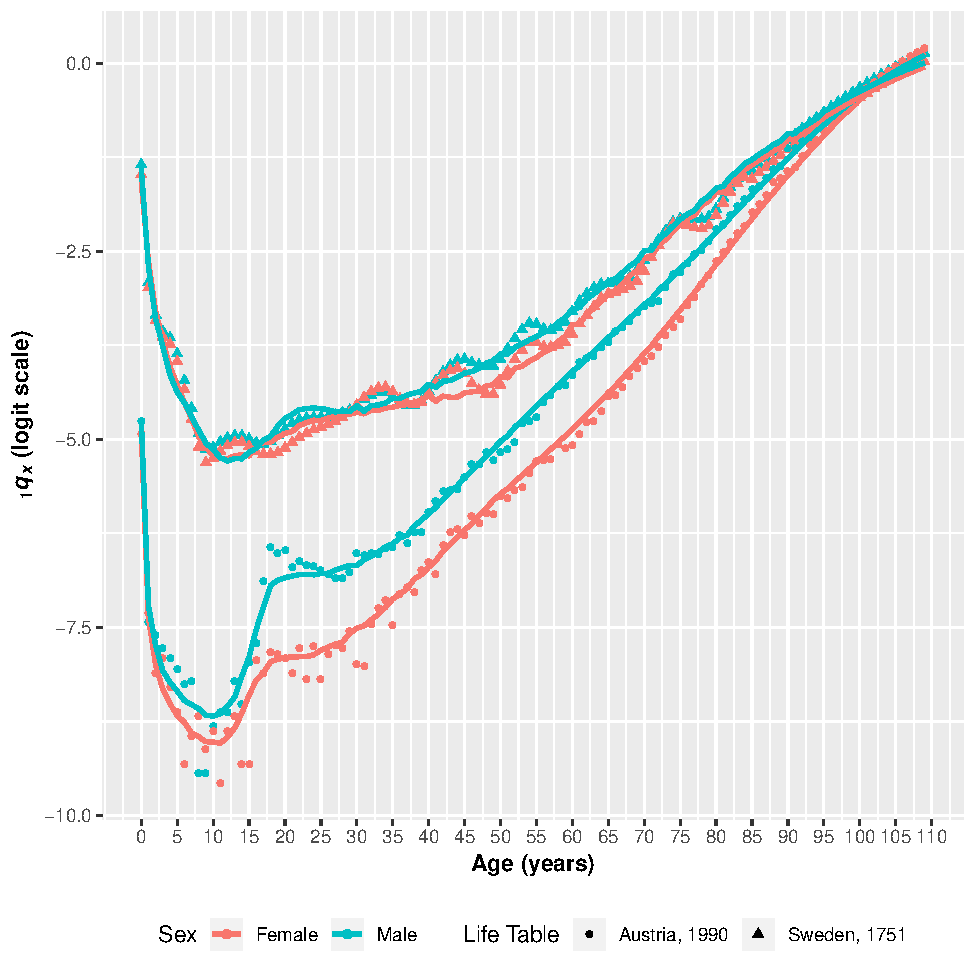
\includegraphics[width=\linewidth]{../figures/fig1.pdf} 
   \captionsetup{format=plain,font=normalsize,margin=0cm,justification=justified}
   \caption{\textbf{Example Data \& Predictions.}  $\qox$ for very high mortality early in Sweden's time series and low mortality for a more recent year in Austria.  Predicted values produced using $\qf$ alone as an input.  Data as symbols and predicted values as lines.}
   \label{fig:data}
\end{figure}

%%% === %%% === %%%
\subsection{Factors of the SVD \label{sec:results:SVDFacs}}

Figure \ref{fig:svd} \added{and Table \ref{tab:appA:comps} in Appendix \ref{app:comps} (on-line appendices)} present the sex-specific LSVs from the SVD of the full set of HMD mortality schedules scaled by their corresponding singular values, $s_{i} \mathbf{u}_{i}$ (ignoring the index for sex $z$).  All elements of $s_1\mbf{u}_1$ are negative so that $s_1\mbf{u}_1$ captures the underlying `average' shape of the mortality profile with age.  Weights applied to $s_1\mbf{u}_1$ move this underlying mortality profile up and down and hence control the overall level of mortality.  The remaining $s_i\mbf{u}_i$ all cross the x-axis and therefore represent age-specific deviations from the overall underlying pattern.  These scaled left singular vectors are the components used in the weighted sum in Equation \ref{eq:colReconU5mr}.  Figure \ref{fig:svd} also displays smoothed\footnote{For components $i \in \{2,3,4\}$, kernel smoother with Gaussian kernel and bandwidth = $i+1$ for ages $i$ and older.} versions of the scaled LSVs.  One can use the smoothed versions to make the predicted mortality schedules smoother.

%%% Figure 2
\begin{figure}[htbp]
   \centering
   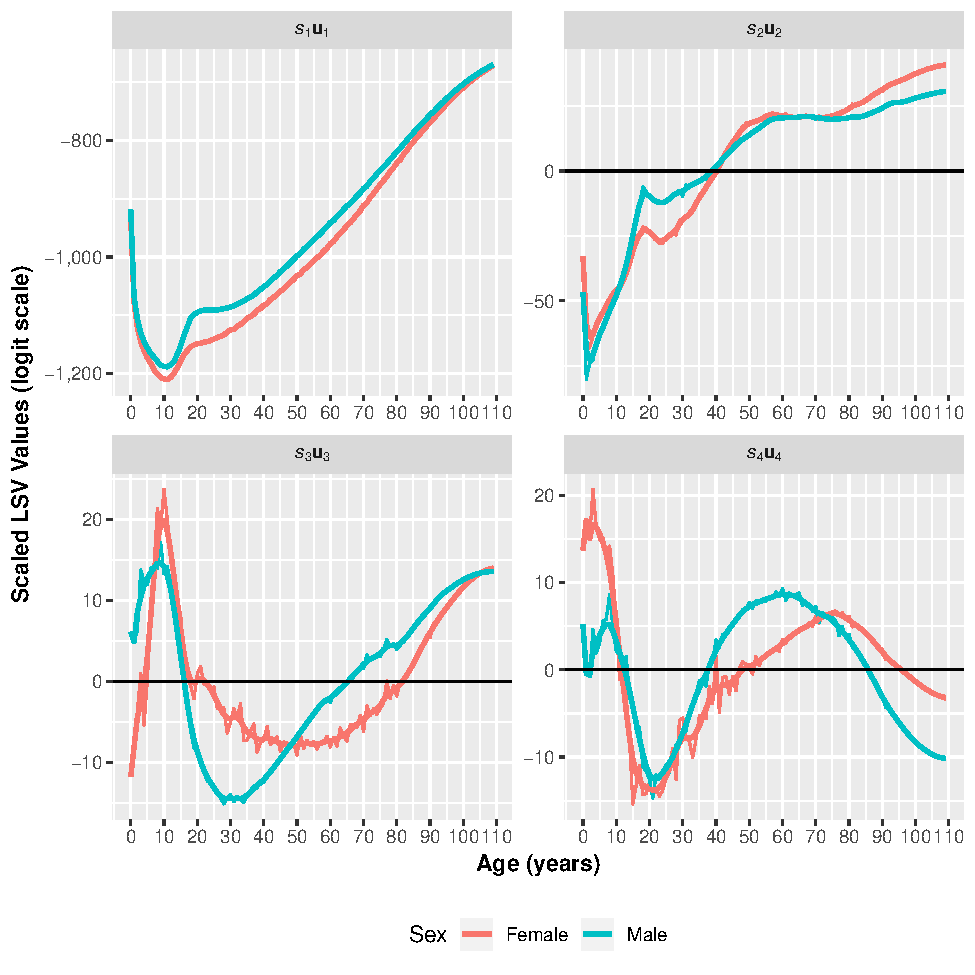
\includegraphics[width=\linewidth]{../figures/fig2.pdf} 
   \captionsetup{format=plain,font=normalsize,margin=0cm,justification=justified}
   \caption{\textbf{Scaled Left Singular Vectors.} First four LSVs scaled by their corresponding SVs from the SVD of the \LTtot mortality schedules in the HMD.  The more variable lines are \textit{raw} components and less variable lines have been smoothed with a kernel smoother.  The raw values are used throughout this work.}
   \label{fig:svd}
\end{figure}

%%% === %%% === %%%
\subsection{Calibration Relationships}

Figures \ref{fig:rsvF} through \ref{fig:q0Child} in Appendix \ref{app:figs} (on-line appendices) display the data and predicted values from the models in Equations \ref{eqn:vsByMx}, \ref{eqn:amCm}, and \ref{eqn:q0Cm}. The corresponding estimated coefficients based on the whole HMD and used to calculate the predicted values in the figures are contained in Tables \ref{tab:appA:femaleRSVMods}, \ref{tab:appA:maleRSVMods}, \ref{tab:appA:adultMxMod}, and \ref{tab:appA:infantMxMod} in Appendix \ref{app:regs}  (on-line appendices).  Figures \ref{fig:rsvF} and \ref{fig:rsvM} in Appendix \ref{app:figs} (on-line appendices) contain scatterplots of the RSV element values versus $\logit(\qf)$.  The figures display both data and values predicted from Equation \ref{eqn:vsByMx} using $\logit(\qf)$ and $\logit(\qff)$ predicted from the model in Equation \ref{eqn:amCm} as inputs.  There are clear, quasilinear relationships between the elements of the RSVs and $\logit(\qf)$. Figure \ref{fig:adultChild} in Appendix \ref{app:figs} (on-line appendices) displays $\logit(\qff)$ versus $\logit(\qf)$, along with the predicted values from Equation \ref{eqn:amCm}.  Finally, Figure \ref{fig:q0Child} in Appendix \ref{app:figs} (on-line appendices) displays $\logit(\qoz)$ versus $\logit(\qf)$, along with predicted values from Equation \ref{eqn:q0Cm}.


%%% === %%% === %%%
\subsection{Cross Validation Prediction Errors} \label{sec:res:crossVal}

Figure \ref{fig:ageSpecErr} displays sex-age-specific boxplots of the error distribution for one-year age groups from the first cross validation using 50 samples of 50\% of the HMD to calibrate the SVD-Comp model.  The errors are generally very small and centered around zero through roughly age 60.  At older ages the size of the errors increases, and the median drifts slightly away from zero in a positive direction, especially at ages older than 90.  However, the median error is never much more than 0.01, and as displayed in Figure \ref{fig:svdVsLqC}, they are significantly smaller than the median errors produced by the Log-Quad model at the same ages.  The error distributions of the in- and out-of-sample predictions are indistinguishable at all ages indicating that the SVD-Comp model is not sensitive to exactly which mortality schedules are used for calibration when half of them are used.

% Figure 7
\begin{figure}[htbp]
   \centering
   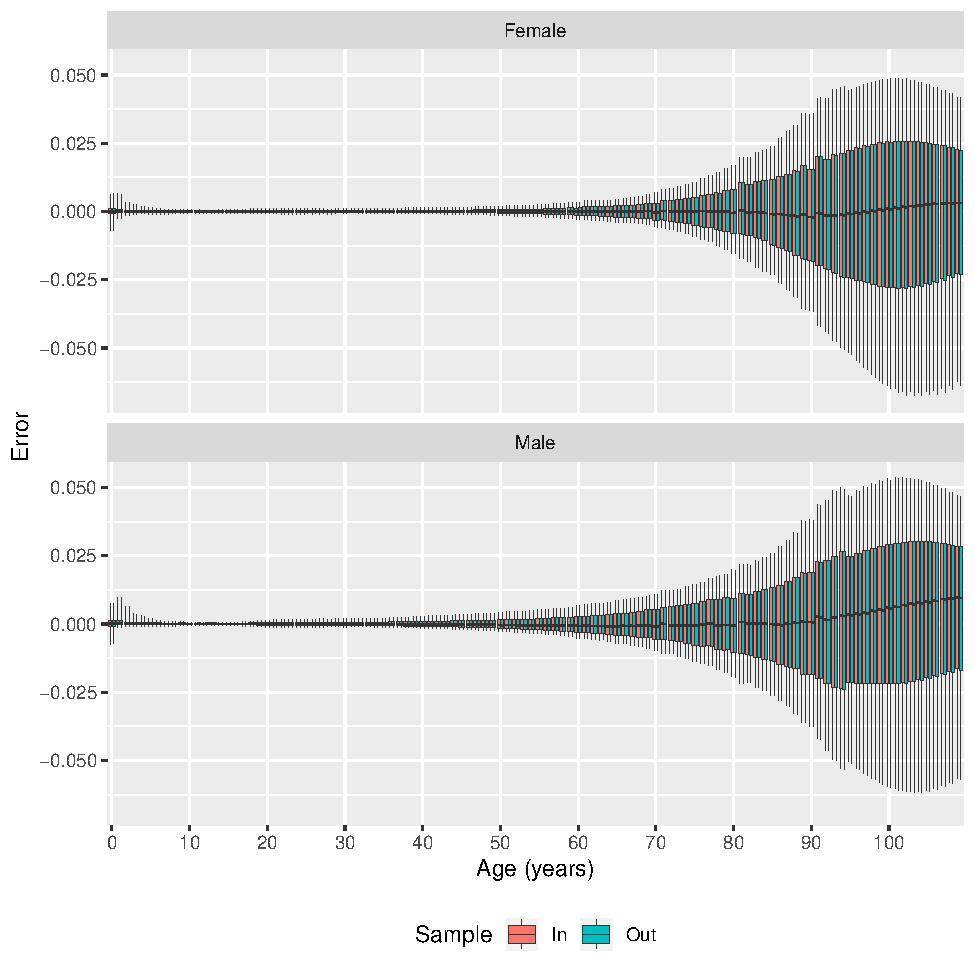
\includegraphics[width=\linewidth]{../figures/fig4.pdf} 
   \captionsetup{format=plain,font=normalsize,margin=0cm,justification=justified}
   \caption{\textbf{SVD-Comp Prediction Errors.}  Single-year age group prediction errors for in- and out-of-sample mortality schedules.  50 50\% samples.  Errors summarized over all in- and out-of-sample mortality schedules for the 50 samples. Whiskers extend to 10\% and 90\% quantiles.}
   \label{fig:ageSpecErr}
\end{figure}

%%% === %%% === %%%
\subsection{Varying Sample Size Cross Validation Prediction Errors} \label{sec:res:sampSize}

Figures \ref{fig:medSampErr} and \ref{fig:iqrSampErr} in Appendix \ref{app:figs} (on-line appendices) contain the second set of cross validation results investigating the effect of varying the number of mortality schedules used to calibrate the SVD-Comp model.  Both figures summarize the overall prediction error distributions (all ages and years combined) for the SVD-Comp model by sample status, in- versus out-of-sample mortality schedules.  The sample fraction varies from 10\% to 90\% in increments of 20\%.   Figure \ref{fig:medSampErr} displays boxplots of the median of medians of overall error.  This is very similar comparing in- and out-of-sample mortality schedules for both sexes across all sample fractions.  There is a slight positive bias in all cases resulting from the positive bias in errors at older ages, see Figure \ref{fig:ageSpecErr}.  A similar situation exists for the distributions of the interquartile range of overall errors, Figure \ref{fig:iqrSampErr} in Appendix \ref{app:figs} (on-line appendices).  The only systematic change in these distributions by sample fraction is that the interquartile range of the indicators calculated from the sample decreases as the sample fraction increases, as expected.  Inversely, there is a weak trend toward increases in the interquartile range calculated in the out-of-sample group as the sample fraction increases, also as expected.  In general the SVD-Comp model appears to be remarkably robust as the number of mortality schedules used for calibration decreases.  Performance is satisfactory all the way down to the 10\% sample and good all all the way down to 30\%.

% Figure 8
\begin{figure}[htbp]
   \centering
   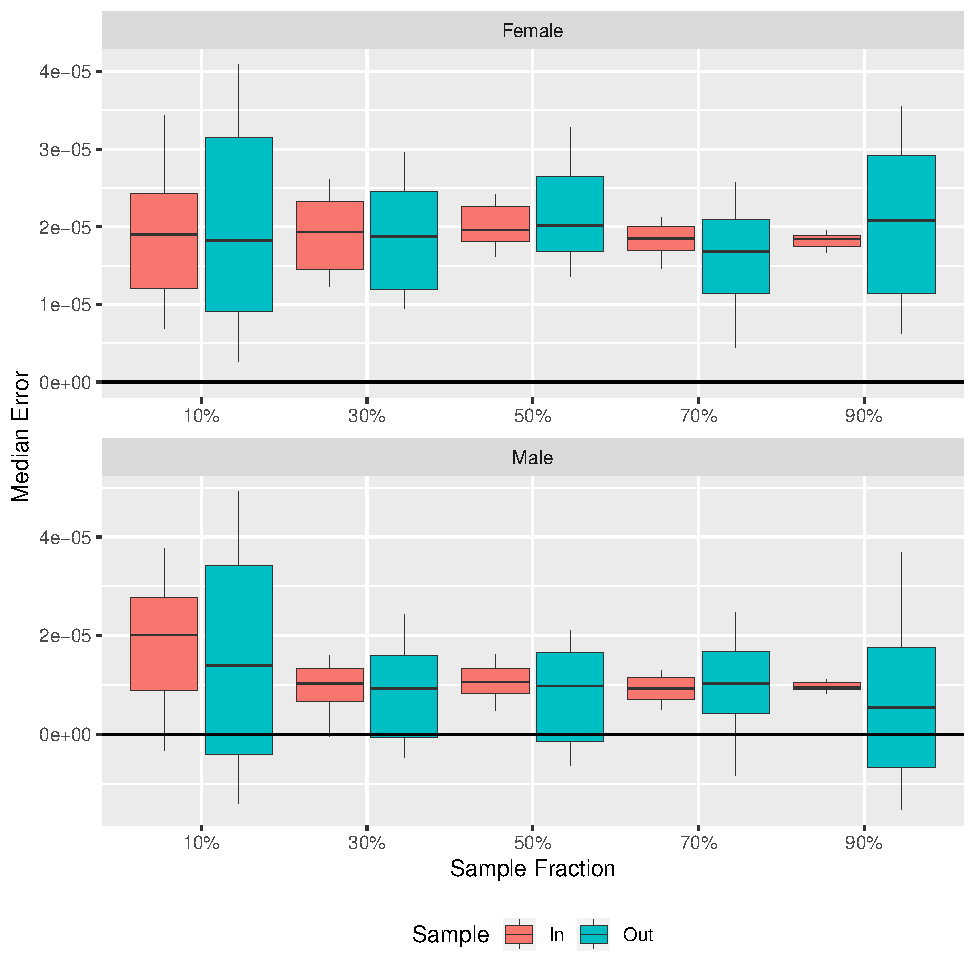
\includegraphics[width=\linewidth]{../figures/fig5a.pdf} 
   \captionsetup{format=plain,font=normalsize,margin=0cm,justification=justified}
   \caption{\textbf{Median Prediction Error by Sample Fraction.}  50 samples for each sample fraction.  For each sample, median calculated across all ages and all mortality schedules in each sample category (in/out). Whiskers extend to 10\% and 90\% quantiles.}
   \label{fig:medSampErr}
\end{figure}

%%% === %%% === %%%
\subsection{Comparison between SVD-Comp and Log-Quad Prediction Errors}

Figure \ref{fig:svdVsLqC} displays sex-age-specific boxplots of the distribution of prediction errors for both the SVD-Comp and Log-Quad models.  The median error by sex and age is close to zero for both models through roughly age 70.  At ages older than 70 the median error for the Log-Quad model is systematically substantially larger than zero, while for the SVD-Comp model the median error stays at zero.  The sex-age-specific interquartile ranges are similar for both models, very small through roughly age 40, growing slowly between 40 and roughly 85 and then shrinking again through 110. In general at ages older than 45 the error distribution for the Log-Quad model is biased in a positive direction, while for the SVD-Comp model the error distribution is centered around zero at all ages.

% Figure 10
\begin{figure}[htbp]
   \centering
   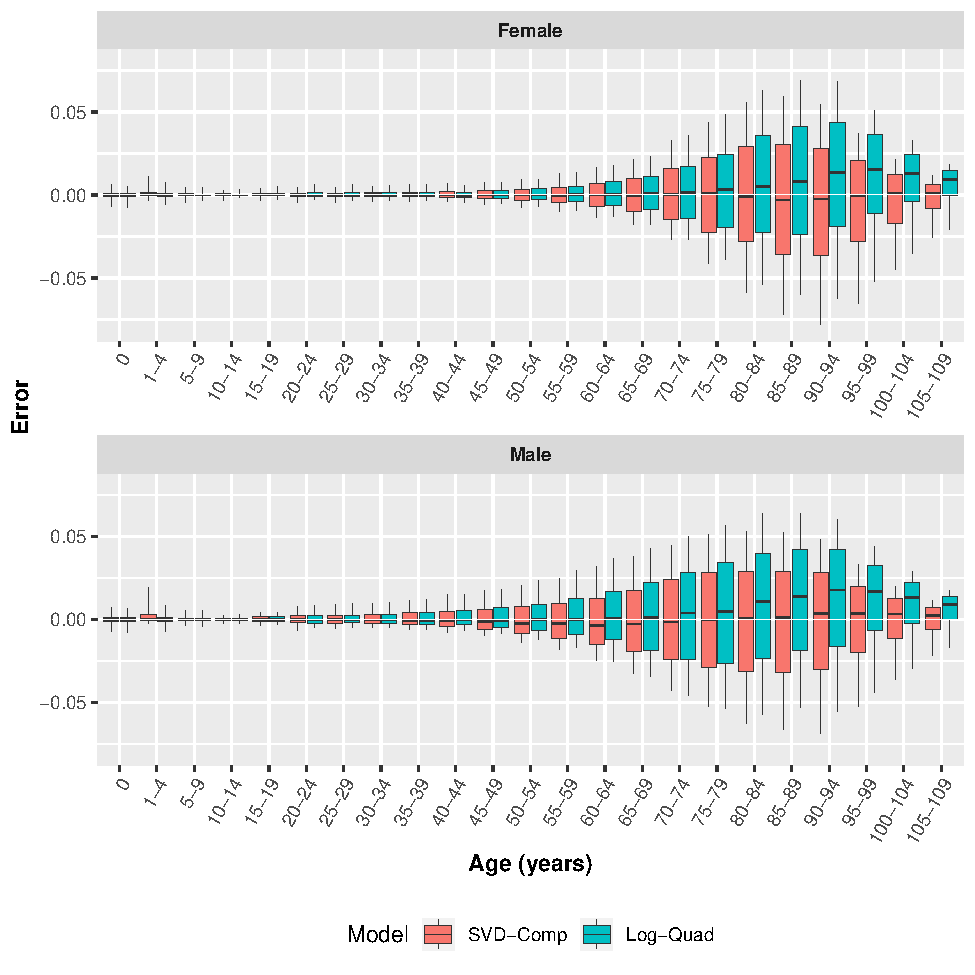
\includegraphics[width=\linewidth]{../figures/fig3.pdf} 
   \captionsetup{format=plain,font=normalsize,margin=0cm,justification=justified}
   \caption{\textbf{SVD-Comp and Log-Quad Prediction Errors.}  Five-year age group prediction errors for SVD-Comp and Log-Quad models using only child mortality $\qf$ as input. Whiskers extend to 10\% and 90\% quantiles.}
   \label{fig:svdVsLqC}
\end{figure}

Table \ref{tab:absErrs} displays the total absolute errors \added{on the natural scale} for the SVD-Comp and Log-Quad models for predictions based on either $\qf$  alone or both $\left(\qf, \, \qff \right)$.  The table also presents differences between the total absolute errors for the two models in both additive (Log-Quad - SVD-Comp) and proportional form ([Log-Quad - SVD-Comp]/SVD-Comp).  In all cases the SVD-Comp model predictions are globally closer to the \replaced{the HMD life tables}{truth}.

\begin{table}[H]
\captionsetup{format=plain,font=normalsize,margin=3cm,justification=justified}
\caption{\textbf{Summary of Prediction Errors for SVD-Comp and Log-Quad.}  Total absolute error and comparisons of total absolute error.  Both models trained on all HMD life tables.}
\begin{center}
\begin{tabular}{llrrr}
\toprule
  &   & \multicolumn{3}{c}{Total Absolute Error Predicted by} \\
\cmidrule{3-5}
 &   & \multicolumn{1}{c}{C1} & \multicolumn{1}{c}{C2} & \multicolumn{1}{c}{C3} \\
 & Model / Summary  & \multicolumn{1}{c}{$\qf$} & \multicolumn{1}{c}{$\left(\qf, \, \qff \right)$} & \multicolumn{1}{c}{C2-C1} \\
 \midrule
\multicolumn{5}{l}{\textit{Female}} \\
 \midrule
 \input{../tables/compsFemale.txt}
 \midrule
\multicolumn{5}{l}{\textit{Male}} \\
 \midrule
 \input{../tables/compsMale.txt}
\bottomrule
\end{tabular}
\end{center}
\label{tab:absErrs}
\end{table}

\added[id=r2]{Tables \ref{tab:qErrs} and \ref{tab:eErrs} in Appendix \ref{app:errorTabs} (on-line appendices) display the weighted sum of age-specific absolute errors in $\widehat{\mbf{q}}_\ell$ and $\widehat{\mbf{e}}_\ell$ across all \LTtot life tables in the HMD. The last row in each displays the sum across all ages.  The unweighted total absolute errors in $\ezhat$ \added[id=editors]{for SVD-Comp calculated using one through four components} are presented in Table \ref{tab:e0Errs} in Appendix \ref{app:errorTabs} (on-line appendices).} \added[id=editors]{Predicted values for life expectancy at birth, $\ezhat$,  reflect predications at all ages so that errors in $\ezhat$ describe the cumulative effect of prediction errors at all ages. With each additional component, the total absolute errors in $\ezhat$ are reduced, and four components are required for SVD-Comp to perform better than Log-Quad. This is true in spite of the fact that the models used to predict the weights for the third and fourth components are not as predictive as those for the weights for the first two components (Equation \ref{eqn:vsByMx} and Tables \ref{tab:appA:femaleRSVMods} and \ref{tab:appA:maleRSVMods} in Appendix \ref{app:regs} (on-line appendices).}

Finally, Figure \ref{fig:preds} in Appendix \ref{app:figs} (on-line appendices) displays predicted $\qox$ from the SVD-Comp using $\qf$ alone for three different levels of $\qf$.

%%% === %%% === %%%
\subsection{Application to Mexico and South Africa}

\added[id=r4]{Figure \ref{fig:mexRSA} displays data and predictions from both Log-Quad and SVD-Comp in standard five-year age groups for Mexico 1983--1985 and South Africa 2005 using both child and adult mortality as predictors.  The two models produce essentially the same predictions for Mexico, and both do an adequate job of following the data given that they are effectively two-parameter models.  The situation for South Africa is different.  As expected neither model is able to follow the HIV/AIDS-related bulge at adult ages.  Both models do a reasonable job of threading the predictions through the male age schedule, overstating the mortality of adolescents and young adults and understating the mortality of middle-aged adults.  For males the predictions are both plausible but unable to reproduce the bulge.  SVD-Comp does the same for females, essentially cutting off the bulge, but Log-Quad produces an implausible age-pattern of mortality with extremely high mortality for older children, adolescents, and young-to-middle-aged adults.  The predictions for South Africa reveal a fundamental limitation of all empirically-based mortality models -- the fact that they cannot represent mortality age profiles that are fundamentally different from those contained in the data used to create them. The solution to this is to identify or create new empirical life tables that represent the age profiles in question and include them in the data used to create the models.}

\begin{figure}[htbp]
   \centering
   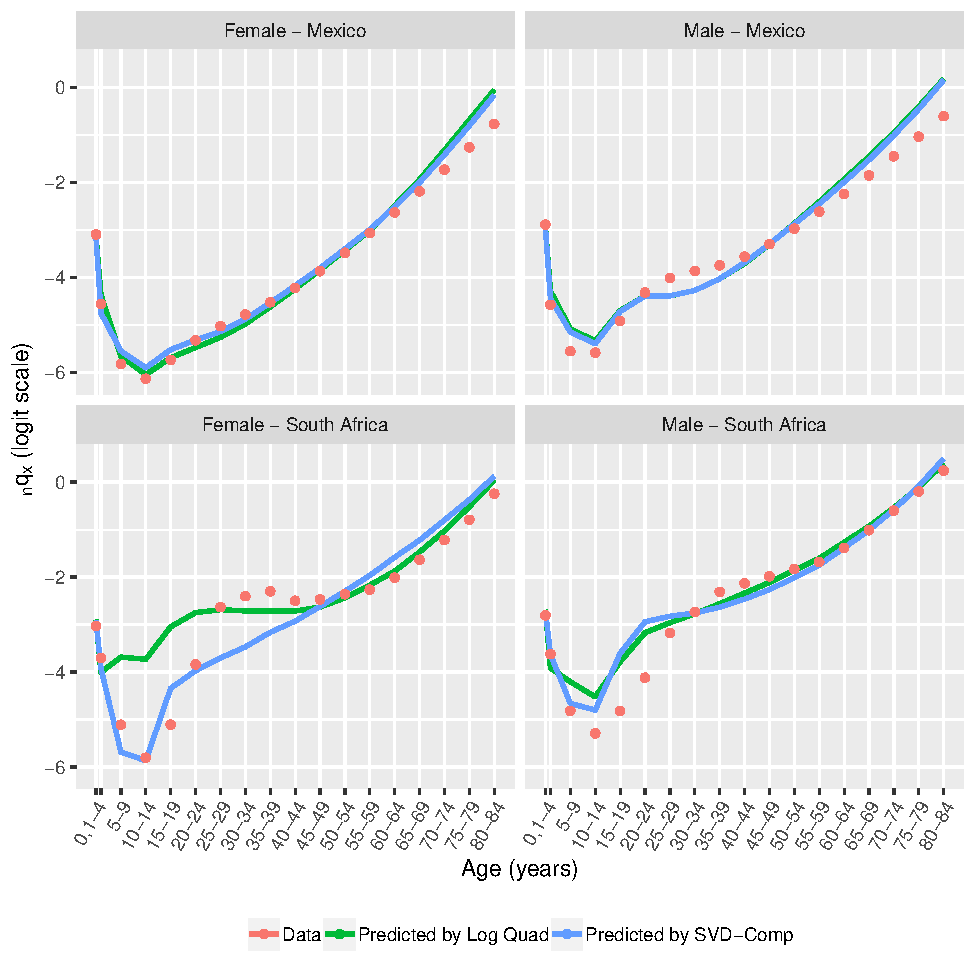
\includegraphics[width=\linewidth]{../figures/fig7.pdf} 
   \captionsetup{format=plain,font=normalsize,margin=0cm,justification=justified}
   \caption{\textbf{Application to Mexico and South Africa.} Data and predicted values in standard five-year age groups produced by Log-Quad and SVD-Comp models using both child and adult mortality as predictors.}
   \label{fig:mexRSA}
\end{figure}


%%% === %%% === %%%
\section{Discussion}

The SVD-Comp model is a simple framework for building mortality models\deleted{that can be either empirical or analytical}.  Its key advantages are
\begin{enumerate*}[label=\arabic*)]
\item a simple linear structure that does not need to be changed to use the model in a variety of ways;
\item a general `interface' through which \replaced{input}{arbitrary} parameters can affect the age pattern of mortality, the weights in Equation \ref{eq:colReconU5mr}; 
\item an ability to handle \replaced{new}{arbitrary} age groups without having to alter the fundamental structure of the model, including very short, like the one-year age groups used here; and finally
\item through its structure, an inherent constraint that ensures that mortality at each age is related to mortality at each other age according to the age patterns reflected in each of the components
\end{enumerate*}.  Along with these, it also satisfies the combined list of desired characteristics for a mortality model enumerated in the introduction.  

This approach is general and allows all-age (in arbitrarily fine age groups) mortality schedules to be predicted from any covariates that are related to age-specific mortality.  This general relationship is quantified in the models (Equation \ref{eqn:vsByMx}) that relate the weights in Equation \ref{eq:colReconU5mr} to the covariates.  Allowing this is the fact that the relationship of each age to all others is maintained through the constant components derived from the SVD, and those intra-age relationships are affected all together through the weights on the components.  This constrains the intra-age relationships and relates them to the covariates in a simple, flexible way.  

When the weights are modeled as functions of child mortality and calibrated using the relationship between the empirical weights ($v_{z \ell i}$ in Equation \ref{eq:colRecon}) and child mortality in the HMD, the model serves the same purpose as the Log-Quad \citep{wilmoth2012flexible} model, and it performs slightly better in a direct comparison, while having the advantage of \added{directly} producing mortality schedules by single year of age. \added[id=r1]{It is important to note that this comparison is conducted with the Log-Quad as presented in \cite{wilmoth2012flexible} and that in that article the authors explicitly favored an estimation technique that would, they claimed, reduce estimation bias at the cost of having (slightly) larger prediction errors when evaluated against the historical dataset, a fact that is apparent in Figure \ref{fig:svdVsLqC}.  The published Log-Quad was calibrated to the slightly different and smaller set of HMD life tables that existed at the time and met the authors' criteria for inclusion.  Consequently the results of the comparison will likely change if the Log-Quad were recalibrated using the same set of HMD life tables described and used here.  However, given how robust the SVD-Comp is to the set of life tables used in calibration (see Sections \ref{sec:res:crossVal} and \ref{sec:res:sampSize}), this potential difference is unlikely to be large.}

\replaced{Concerning calibration and complexity, t}{T}he cross validation results clearly demonstrate that the calibration to the HMD is robust with respect to exactly which and how many mortality schedules are used\replaced[id=r2]{, and SVD-Comp is no more complex than Log-Quad.}{Finally, the} SVD-Comp\deleted{model} \replaced{requires}{uses} \added[id=r2]{one SVD calculation and} six regression models (four in Equation \ref{eqn:vsByMx}, one in Equation \ref{eqn:amCm}, and one in Equation \ref{eqn:q0Cm}) for each sex to capture the relationship between child mortality and mortality at other ages in the HMD \added{- 12 regression models in total}.  \deleted{In contrast the} Log-Quad \replaced{requires}{uses} \added[id=r2]{one SVD calculation and} one log-quadratic model of the general form $\log(\mfx) \sim \log(\qf) + \log(\qf)^2$ for each five-year age group and another to refine the prediction of $\qoz$ for each sex -- 46 regression models in total.  \added[id=r2]{The total number of regression coefficients required by each model (for each sex) is: 44 for SVD-Comp and 70 for Log-Quad.  The total number of discrete values required for prediction (for each sex) is: SVD-Comp - 484 (4.4/age group), and Log-Quad - 92 (3.8/age group).  The models directly predict mortality in: SVD-Comp - single-year age groups, and Log Quad - five-year age groups.  Comparing the complexity of the models is not easy and depends where one focuses, but it is clear that neither is obviously more/less complex than the other.  Perhaps the only important difference in this respect is that there is nothing in the overall Log-Quad model to directly constrain the relationship of mortality at one age to another except for the quadratic form of the relationship between mortality at each age and $\qf$, whereas SVD-Comp manipulates a linear combination of age-specific vectors, so the relationships between ages are constrained to fall within the four-dimensional space defined by the four components used by SVD-Comp.}  

Together with our earlier work on an HIV-calibrated version of SVD-Comp  \citep{sharrow2014modeling}, this demonstration suggests that it is reasonable to expect that SVD-Comp could be calibrated in a variety of additional ways to produce useful models that relate age-specific mortality to, for example, life expectancy at birth (or some other age), GDP, geographic region, time period, epidemiological indicators \citep[as in ][]{sharrow2014modeling}, a combination of any of these, or something else.  Moreover, subtle effects on the age structure of mortality such as the `rotation' in age-specific mortality identified by \cite{li2011} could be incorporated by adding the necessary elements to the models for the weights.  The same approach could be applied to develop models for the difference between underlying age-specific mortality and age-specific mortality affected by specific shocks such as natural disasters, conflict or epidemic disease such as HIV.  It is even possible to refine the Lee-Carter model in Equation \ref{eq:leeCarter} by adding more components to the SVD-derived $\mbf{b}_xk_t$ term so that the enhanced model could represent a wide range of age patterns instead of the constant age pattern included in the existing formulation.  This would add more parameters to the model, but the payoff might be sufficient to make that worthwhile.  Going further, the entire Lee-Carter model could be replaced by the SVD-Comp model which would give it the ability to model changing levels and age patterns of mortality independently and generally be more flexible.

The general SVD-Comp model in Equation \ref{eq:colReconU5mr} can be used in another way to interpolate or smooth incomplete or noisy age schedules by simply using OLS regression of the incomplete mortality schedule against the corresponding elements of the first few components $s_{zi}\mbf{u}_{zi}$ with the constant constrained to be zero, and then predicting the full mortality schedule from all elements of the components and the coefficients estimated by the regression.   Bayesian estimation can also be used to estimate the weights and their uncertainty, similar to \cite{Sharrow_29_39}.

\added[id=r4]{The application to Mexico and South Africa confirmed that the HMD-calibrated SVD-Comp works at least as well as Log-Quad when applied to mortality schedules in populations well outside of the HMD.  For South Africa neither model was able to reproduce the HIV/AIDS-related mortality bulge at adult ages.  SVD-Comp produced plausible mortality schedules for both sexes that were as close as possible to South Africa's, given that it could not reproduce the bulge.  In contrast, Log-Quad produced a plausible mortality schedule for males but a nonsensical schedule for females.  These results reveal an urgent need to increase the diversity of mortality schedules available in freely-accessible archives like HMD, and in particular, an important need to compile much better mortality data for Africa and other developing world regions where age schedules of mortality are different from what has been observed in the developed world.  Additionally, the South Africa application suggests that SVD-Comp may provide a stable framework to begin building mortality models that include epidemiological (e.g. HIV prevalence and ART coverage) and other predictors.  Our earlier work using modeled data \citep{sharrow2014modeling} is a start, but building models using modeled data is of limited value so we must assemble reasonable large, high quality empirical mortality data sets from the places where models such as Log-Quad and SVD-Comp are most useful.}


%%% === %%% === %%%
\section{Software \& Reproducibility Materials}

There is a GitHub repository containing all the code necessary to reproduce the results presented in this manuscript: \url{https://github.com/sinafala/svd-comp}.  The on-line version of this article includes both the on-line appendices and a PDF rendered from the R Markdown file (on GitHub) that produces the results.

An \textsf{R} package \citep{RCore} implementing the HMD child or child/adult mortality-calibrated version of SVD-Comp presented above is available as fully open source and free software to download directly from the GitHub repository using the \textit{devtools} R package and command: 
\begin{verbatim}
install github(repo = "sinafala/svdComp5q0")
\end{verbatim}


%%% === %%% === %%%
\section*{Acknowledgements}

This work was supported in part by grant R01 HD054511 from the Eunice Kennedy Shriver National Institute of Child Health and Human Development (NICHD).  The funder had no part in the design, execution, or interpretation of the work.  Tables of regression coefficients are formatted using the LaTeX package `stargazer' \citep{stargazer}.  


\newpage
%%% === %%% === %%%
\addcontentsline{toc}{section}{References}
\bibliography{SVD-Comp}
\bibliographystyle{demography}

\end{document}  